\subsection*{Data acquisition}
We recorded the calcium activity  of dense populations of neurons in the supragranular layers in primary visual cortex of anesthetized mice using fast random-access 3D scanning two-photon microscopy \cite{Stosiek:2003,Reddy:2005}.  Numerious repetitions of full-field drifting gratings (Fig. 1A and 1B) were presented to the eye contralateral to the imaged site. This technique allowed recording from a large number (150--350) of cells in a small volume of cortical tissue ($200\times200\times100$ $\mu$m$^3$) in layers 2/3 and 4. Somatic calcium signals were deconvolved using  sparse nonnegative deconvolution \cite{Vogelstein:2010} (Fig. 1C and 1D).  The average stimulus response was subtracted to remove stimulus covariance and the sample noise covariance matrix was computed (Fig. 1E).

\begin{figure}[!ht]
\begin{center}
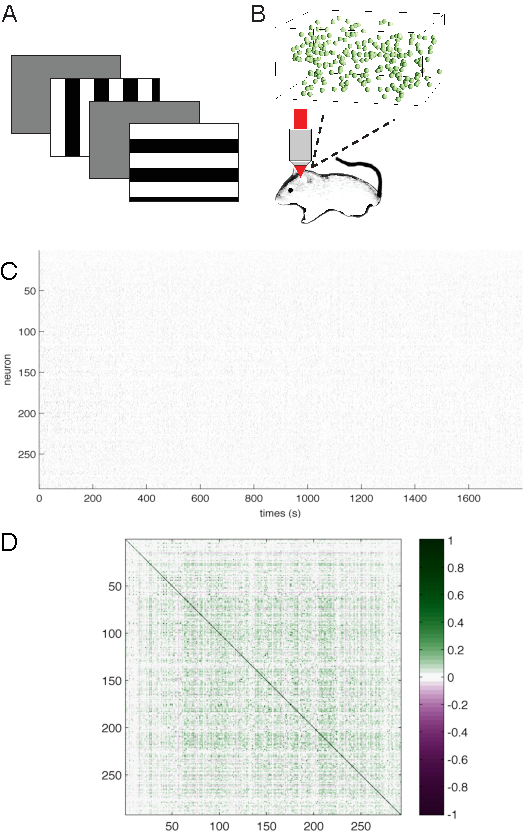
\includegraphics[width=4in]{figures/Figure1.pdf}
\end{center}
\caption{
{\bf Acquistion of neural population activity using two-photon fluorescence imaging of calcium signal.}  {\tt A.} Visual stimuli comprising brief (500 ms) presentatios of full-field drifting gratings separated by blank screens. {\tt B.} Two-photon fast 3D imaging of calcium signals in an awake mouse. {\tt C.} Deconvolved calcium signals. {\tt D.} The sample covariance matrix of neuronal calcium signals in 200 ms time bins. 
}
\label{Figure_label}
\end{figure}


\subsection*{Sample covariance matrix}
We aim to estimate the true covariance matrix $\Sigma = \mathbb E [(x-\mu)(x-\mu)^\T]$ , where $\mathbb E[\cdot]$ denotes expectation \TODO{under the true model}, $x$ denotes the $p\times 1$ vector of real-valued instanteous firing rates of $p$ neurons in a bin of duration $\Delta t$ and $\mu = \mathbb E[x]$.  For more rigourous notation, definitions, and derivations, see Appendix. 

The usual estimator of $\Sigma$ is the sample covariance matrix
\begin{equation}
\hat \Sigma_0 = \frac 1 {n-c} \sum\limits_{t=1}^n (x(t)-\mu)(x(t)-\mu)^\T 
\end{equation}
where $x(t),\;t=1,\ldots,n$ are sequential observations of population activity inferred from calcium signals. Bessel's correction $c$ makes the estimate unbiased such that $\mathbb E[\hat\Sigma_0] = \Sigma$. When observations $x(t)$ can be assumed to be independent then $c=1$; but when observations are correlated $c>1$ may be estimated from the data. 

\subsection*{Regularized estimates of the covariance matrix}
To assess the quality of a covariance matrix estimate $\hat\Sigma$, we must define a real-valued \emph{loss function} $\mathcal L(\hat\Sigma,\Sigma)$, which attains its minimum when $\hat\Sigma = \Sigma$. For the purposes of this study, we adopted the \emph{Gaussian loss} function:
\begin{equation}
\mathcal L(\hat\Sigma,\Sigma) = \mathcal L_g(\hat\Sigma,\Sigma) = \frac 1 p(\ln \det \hat \Sigma + \Tr(\hat \Sigma^{-1}\Sigma))
\end{equation}
which resembles the negative multivariate normal log-likelihood (see Appendix).
 

Although the sample covariance matrix is unbiased: $\mathbb E[\hat\Sigma_0]=\Sigma$, it is not as close to $\Sigma$ as possible, on average. We must seek  to minimize the expected value of the loss function, known as \emph{estimator risk} 
\begin{equation}
r = \mathbb E[\mathcal L(\hat\Sigma, \Sigma)]
\end{equation}

Estimator risk can be reduced by \emph{regularization}. Regularization is the deliberate biasing (\emph{``shrinkage''}) of the estimate toward a low-dimensional, less variable \emph{target estimate} \cite{Bickel:2006,Ledoit:2004}.  Resulting regularized estimators are biased but  less variable. Regularization procedures must strike favorable balance between bias and variance so that the estimator risk is minimized. The terms \emph{bias} and \emph{variance} are applicable only the loss function is mean-squared-error. The more general terms are \emph{approximation error} and \emph{estimation error})

Numerous regularized covariance matrix estimates have been devised. They start with the sample covariance matrix but differ in the choice of the target estimate and the shrinkage path and intensity. Some regularization schemes focus on the optimal choice of the low-dimensional target estimate from a large family of target estimates and do not require shrinkages.  Others have a fairly simple target estimate but instead adjust the shrinkage intensity to reduce the estimation error.

A regularized estimate of $\Sigma$ can be constructed by either (a) selecting an optimal low-dimensional approximation of $\hat\Sigma_0$ from a given family of approximations and/or (b) biasing or \emph{shrinkage} of $\hat\Sigma_0$ toward a given low-dimensional target estimate by an optimal amount.  Both dimensionality reduction and shrinkage approaches reduce the variance of the solution while introducing bias. 


We evaluated four regularized estimators which we will denote as A, B, C, and D.  Their target estimates correspond to covariance matrices of Gaussian graphical models depicted in Figure 2.  Here the green spheres represent the recorded neurons. The light-colored balls represent latent units of the graphical model and the edges connecting them represent conditional dependencies.

\begin{figure}[htp]
\centering
\includegraphics[width=0.5\textwidth]{figures/Figure2.pdf}
\caption{
Graphical models corresponding to the low-dimensional targets of the four regularization schemes used in the paper. It assumed that all interactions are linear, \emph{i.e.}\;the mean firing rate of any neuron can be computed by a linear combination of the firing rates of other neurons and latent units.
\textbf{A}: ``Independent.'' A population with no interactions corresponds to the diagonal covariance matrix.
\textbf{B}: ``Latent factors.'' Observed nodes are assumed to be influenced by several latent units (``factors") but are otherwise independent.
\textbf{C}: ``Sparse.'' Partial correlations between a subset of pairs of observed neurons, zero partial correlations between all other pairs.  
\textbf{D}: ``Sparse+latent.''  Partial correlations between a subset of pairs of observed neurons and a few latent factors interacting with the entire population. 
}\label{fig:02}
\end{figure}


A \emph{graphical model} is a multivarate probability distribution with a specified graph of conditional dependencies between its variables \cite{Koller:2009}.  When such a distribution is a multivariate normal distribution, the model becomes a \emph{Gaussian graphical model} or, equivalently, a \emph{Gaussian Markov Random Field}.  Gaussian graphical models have a straightforward relationship to their covariance matrix $\Sigma$:  Zero elements in the inverse of $\Sigma$ indicate conditional independence between the corresponding pair of variables.  

Fitting a graphical model to data involves two tasks: (1) the selection of the set of non-zero covariances or \emph{covariance selection} \cite{Dempster:1972} and (b) the fitting of the non-zero elements.

\subsubsection*{Estimate A: Shrinkage toward the independent model}
In estimate A, the target is a family of diagonal matrices 
\begin{equation}
\hat T_\alpha = (1-\alpha)(\hat\Sigma_0 \circ I) + \frac \alpha p \mbox{tr}(\hat \Sigma_0)I
\end{equation}
where $\circ$ is the entrywise product (Hadamard product). When $\alpha=0$, $\hat T_\alpha$ has the average variance along the diagonal. When $ \alpha=1$, $ \hat T_\alpha$ has empirical variances on the diagonal.

If dependencies between neurons are strictly linear, then a diagonal covariance matrix represents the case where neurons are independent, with no interactions.

The overall estimate $\hat\Sigma$ is found by linear mixing of $\hat\Sigma_0$ and $ \hat T_\alpha$ controlled by the mixing proportion $\lambda$:
\begin{equation}
\hat\Sigma = (1-\lambda)\hat\Sigma_0 + \lambda\hat T_\alpha 
\end{equation}

The hyperparameters $ \alpha$ and $ \lambda$ can be optimally selected from the training data by nested cross-validation.

\subsubsection*{Estimate B: Shrinkage toward }
In estimator B, the target is the multifactor model $ \hat T_d$ with $ d$ latent units. When all dependencies are linear, factor models correspond to mutually independent neurons each influenced by $ d$ latent units. (This is  the conventional factor analysis).

Just as in A, the overall estimate is found by linear mixing:
\begin{equation}
\hat\Sigma = (1-\lambda)\hat\Sigma_0 + \lambda\hat T_d
\end{equation}

\subsubsection*{Estimate C}
In estimate C, the target $ \hat S_\alpha$ is a matrix whose inverse is \emph{sparse}, with a large fraction of off-diagonal elements fixed at zero. The coefficient $ \alpha$ controls the sparsity in $ \hat S_\alpha$.

In models with only linear dependencies, zeros in the inverse covariance indicate conditional independence. Thus the target estimate is depicted as the graphical model with sparse interneuronal interactions.

In practice the target $\hat S_\alpha$ is found by an $ L_1$-norm optimization technique, which combines dimensionality reduction and shrinkage into a single computationally efficient algorithm.

Just as in the previous estimators, the optimal value of the regularization parameter $ \alpha$ is determined from the data by nested cross-validation.

\subsubsection*{Estimate D}
In estimate D, the target $\hat R_{d,\alpha}$ is the matrix whose inverse is the sum of a sparse matrix $\hat S_\alpha$ and a low-rank matrix $\hat L_d$ of rank $d$.
\begin{equation}
\hat R_{d,\alpha} = (\hat S_\alpha + \hat L_d)^{-1}
\end{equation}

If all dependencies are linear, the estimate D describes a group of neurons where each interacts with a small number of latent units and a small fraction of the observed neurons. 

\subsection*{Sparse inverse covariance with a low-rank component dominates other estimators}
I computed noise covariances of population activity from 31 sites.  In each site, I compared the cross-validated performance of the covariance matrix using the Gaussian log-likelihood loss function between the trained estimate $ \hat\Sigma$ and the testing sample covariance $ \Sigma_0^\prime$:
\begin{equation}
\mathcal L(\hat\Sigma,\hat\Sigma_0^\prime) = 
\frac 1 p\left( \ln \det \hat \Sigma + \mbox{tr}(\hat \Sigma^{-1}\hat\Sigma_0^\prime) \right) 
\end{equation}

I obtained the following in figure 3.

This is the full matrix of all comparisons of the estimators.  The plots represents the histograms of the differences of the loss function between the pair of estimators for all 31 sites.  When the differences are positive, the first estimate in the title outperforms the second estimate.

Of particular interest is the first row, which shows that all regularized estimates  outperformed the sample covariance estimate.  Even more informative is the last column, which shows that estimate D (sparse+lowrank) significantly outperformed all other estimates.



